\section{Информационные метрики}
\subsection{Случай без сужения пространства}
Для оценки метрики 
\begin{gather}
\begin{aligned}
min_{Z} I[X, Z] - \beta * I[Z, Y]
\end{aligned}
\end{gather} 
требуется считать совместные информационные эвристики между латентным пространством и входным/выходным, вспомим формулу информации между латентным пространством $Z$ и входным пространством $X$
\begin{gather}
\begin{aligned}
    I[X, Z] = - \EX_{p(x, z)}\log(\frac{p(x)p(z)}{p(x, z)}) = \\ \sum_{i=0}^{len\_dataset}p_{XZ}(x=x_i, z=z_i) * \log(\frac{p_{XZ}(x=x_i, z=z_i)}{p_X(x=x_i) * p_Z(z=z_i)})
\end{aligned}
\end{gather}    
где 
\begin{gather}
\begin{aligned}
p_X(x=x_i) = count(discrite(x_i)) / len(dataset) \\
p_Z(z=z_i) = count(discrite(z_i)) / len(dataset) \\
p_{XZ}(x=x_i, z=z_i) = count(concat(discrite(x_i), discrite(z_i))) / len(dataset) 
\end{aligned}
\end{gather}
То есть мы считаем количество элементов эдементов в датасете которые перешли в одни и те же дискретные исходы и на основе этих количеств строим вероятностное пространство. Заметим что свойства вероятностной меры соблюдены: сумма всеъ вероятностей равна 1, мера не отрицательна, соблюдедается аддитивность. \\
Аналогично считается $I[Y, Z]$:
\begin{gather}
\begin{aligned}
    I[Y, Z] = - \EX_{p(y, z)}\log(\frac{p(y)p(z)}{p(y, z)}) = \\ \sum_{i=0}^{len\_dataset}p_{YZ}(y=y_i, z=z_i) * \log(\frac{p_{YZ}(y=x_i, z=z_i)}{p_Y(y=y_i) * p_Z(z=z_i)})
\end{aligned}
\end{gather} 
только при этом не происходит дискретизация для $Y$, тк оно и так принимает целые значения от 0 до 9. \\
Соответственно если рассматривать пространства $p_{XZ}, p_{YZ}, p_{X}, p_{Z}$ без сужения велика вероятность получения равномерного распределения независимо от латентного пространства, то есть 
\begin{gather}
\begin{aligned}
p_X(x=x_i) = \frac{count(discrite(x_i))}{len(dataset)} \approx \frac{1}{len(dataset)} \\
p_Z(z=z_i) = \frac{count(discrite(z_i))}{len(dataset)} \approx \frac{1}{len(dataset)} \\
p_{XZ}(x=x_i, z=z_i) = \frac{count(concat(discrite(x_i), discrite(z_i)))}{len(dataset) } \approx \frac{1}{len(dataset)} 
\end{aligned}
\end{gather}
Это будет для больших пространств пространств, таких как входной слой или первые слои свертки, где также много параметров. Дело в том, что дискретизация в таких случаях будет инъективным отображением как на входном пространстве, так и на латентном, также функция преобразования (часть forward pass) будет инъективной, а значит выполняются такие апроксимации для любых латентных пространств независимо от эпохи обучения. Соответветственно информация будет константной и не будет менятся от эпохи обучения, как и метрика Information Bottleneck (15). \\
Соответственно для решения этого нам потребуются уменьшение вероятностных пространств, чтобы избавится от инвариантоности и сделать распределение неравномерным. Также без сужение пространства построение вероятностного пространства и подсчет информационных метрик ресурсно затратно, так как требуется хранить большой сет и итерироваться по нему, что долго. \\
Представим инфмаорционные метрики на графиках в зависимости от эпохи обучения. Всего было 10 эпох обучения, в каждой из итераций строилось новое вероятностное пространство и по нему считались давнные эвристики.
\begin{center}
    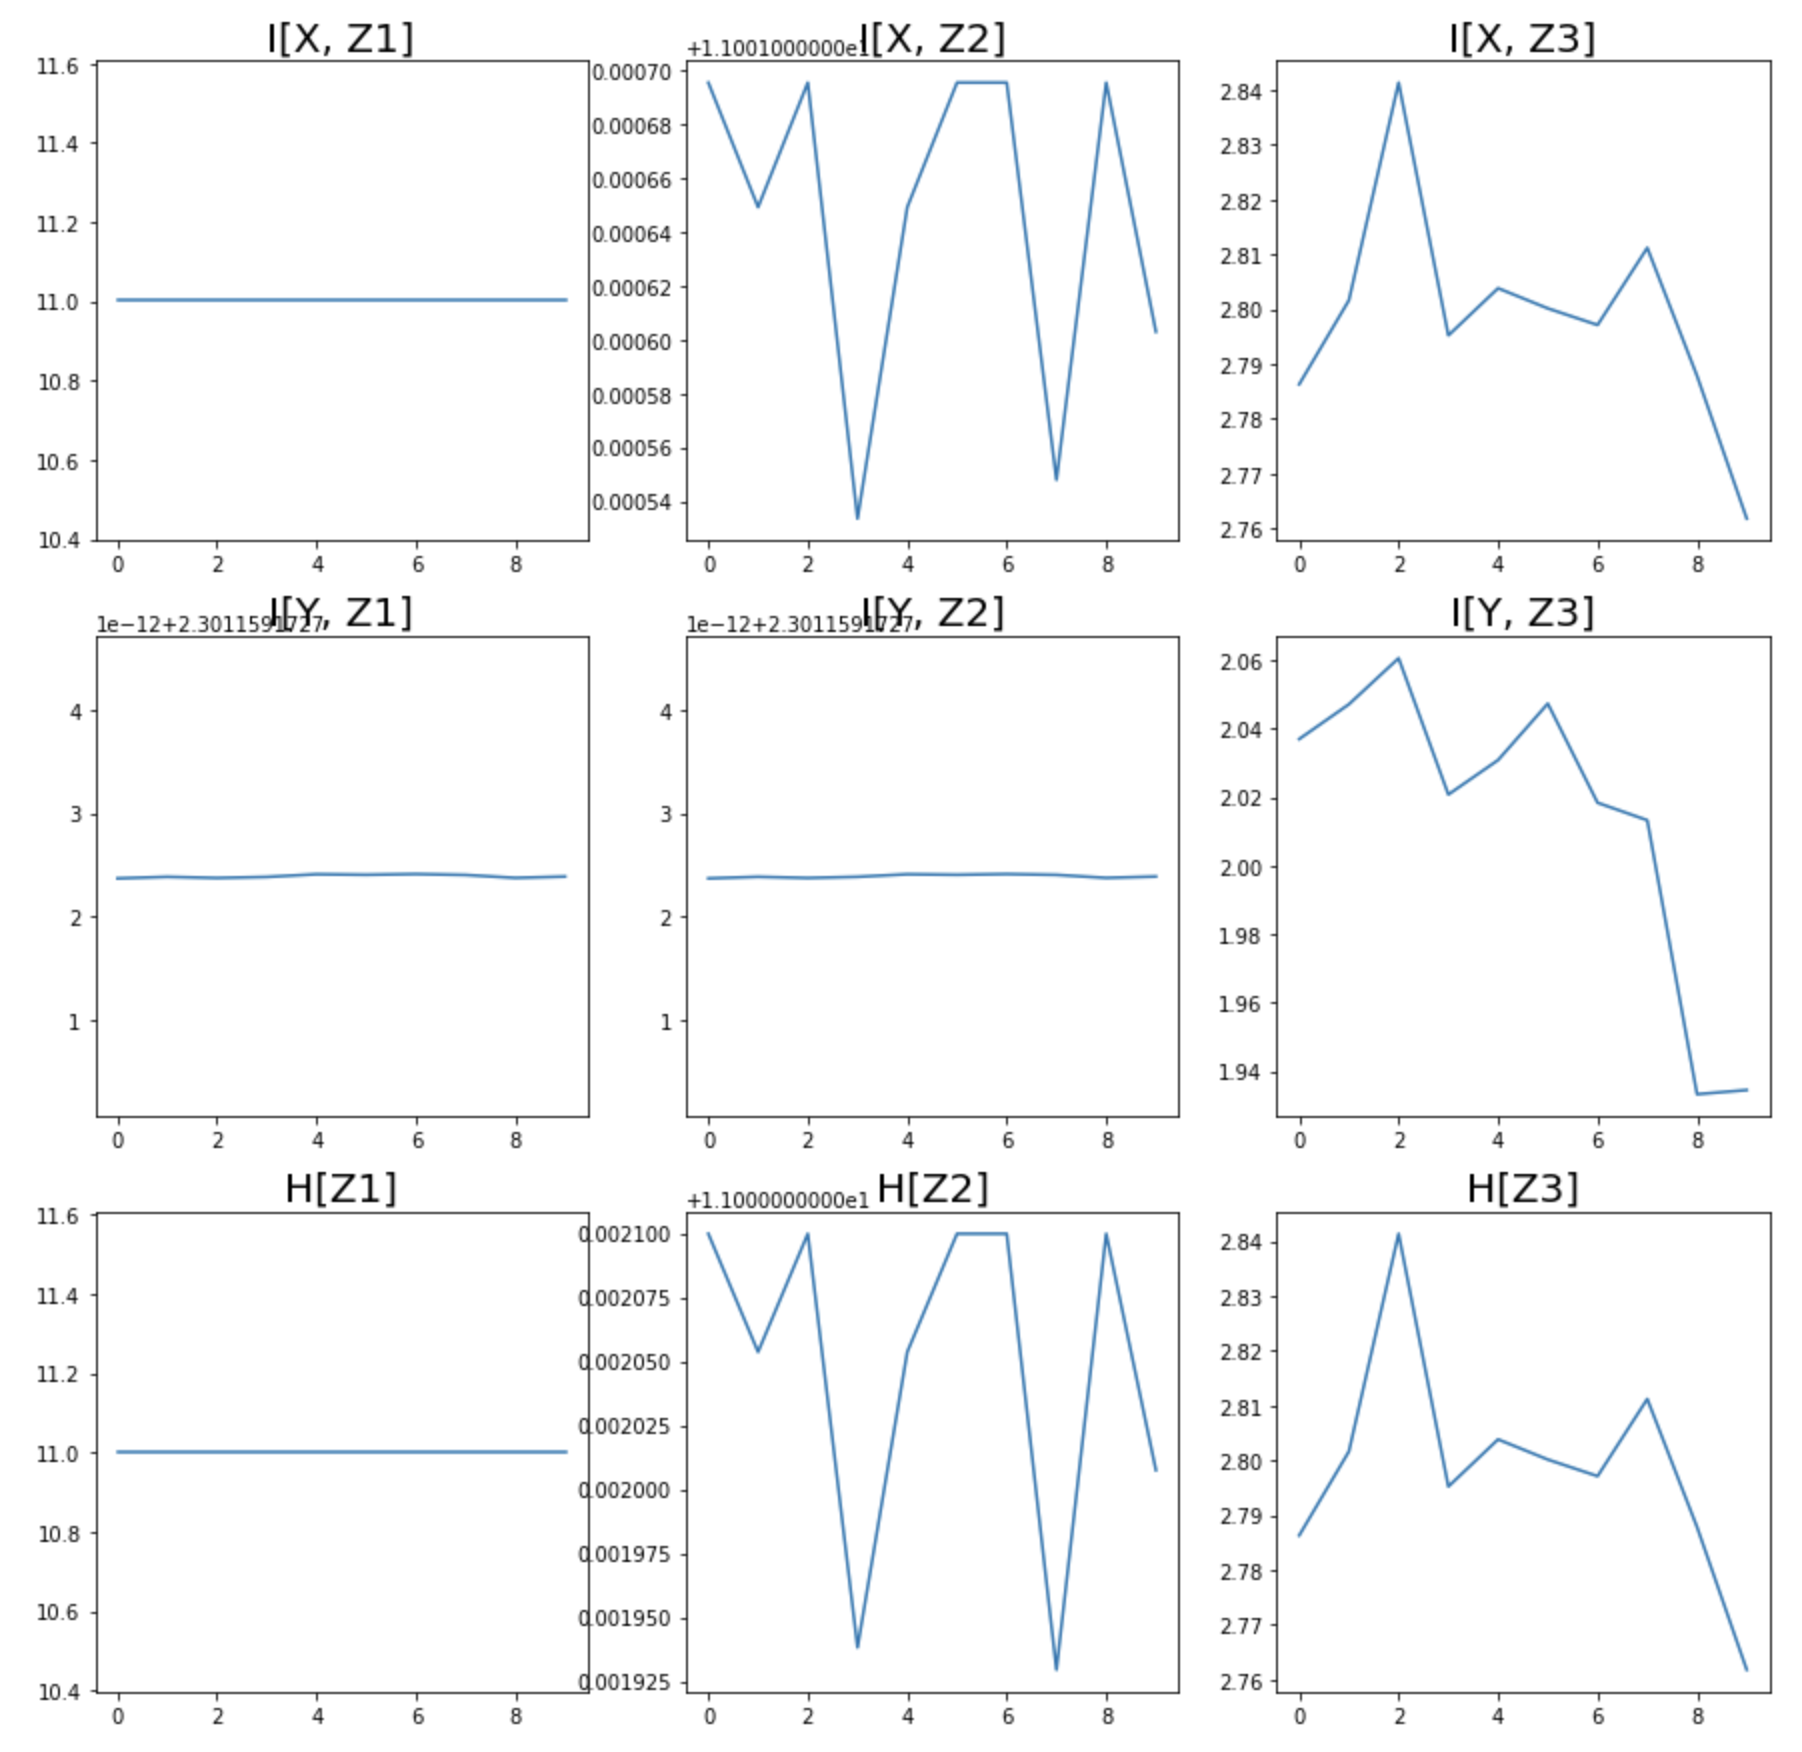
\includegraphics[scale=0.45]{images/inf_without_comp.png}
\end{center}
Как можно заметить $H[Z_1], I[X, Z_1], I[Y,Z_1]$ статичны независимо от эпохи. Это происходит из-за того что построенные вероятностные пространства распределены равномерно, это еще раз подтверждает то, что латентное пространство требуется сужать. Также метрики не имею никакую тенденцию. Мы пришли к выводу что задача нейронной сети уменьшение эвристики: 
\begin{gather}
\begin{aligned}
I[X, Z] - \beta * I[Z, Y]
\end{aligned}
\end{gather}
Здесь же не наблюдается уменьшение метрики $I[X, Z]$ и увеличение метрики $I[Y, Z]$ ни для ни одного латентного пространства $Z_1, Z_2, Z_3$.
\subsection{Случай сужения пространства}
Рассмотрим пример с сужением вероятностных пространств и посчитаем на них аналогично информационные эвристики в зависимости от эпохи:
\begin{center}
    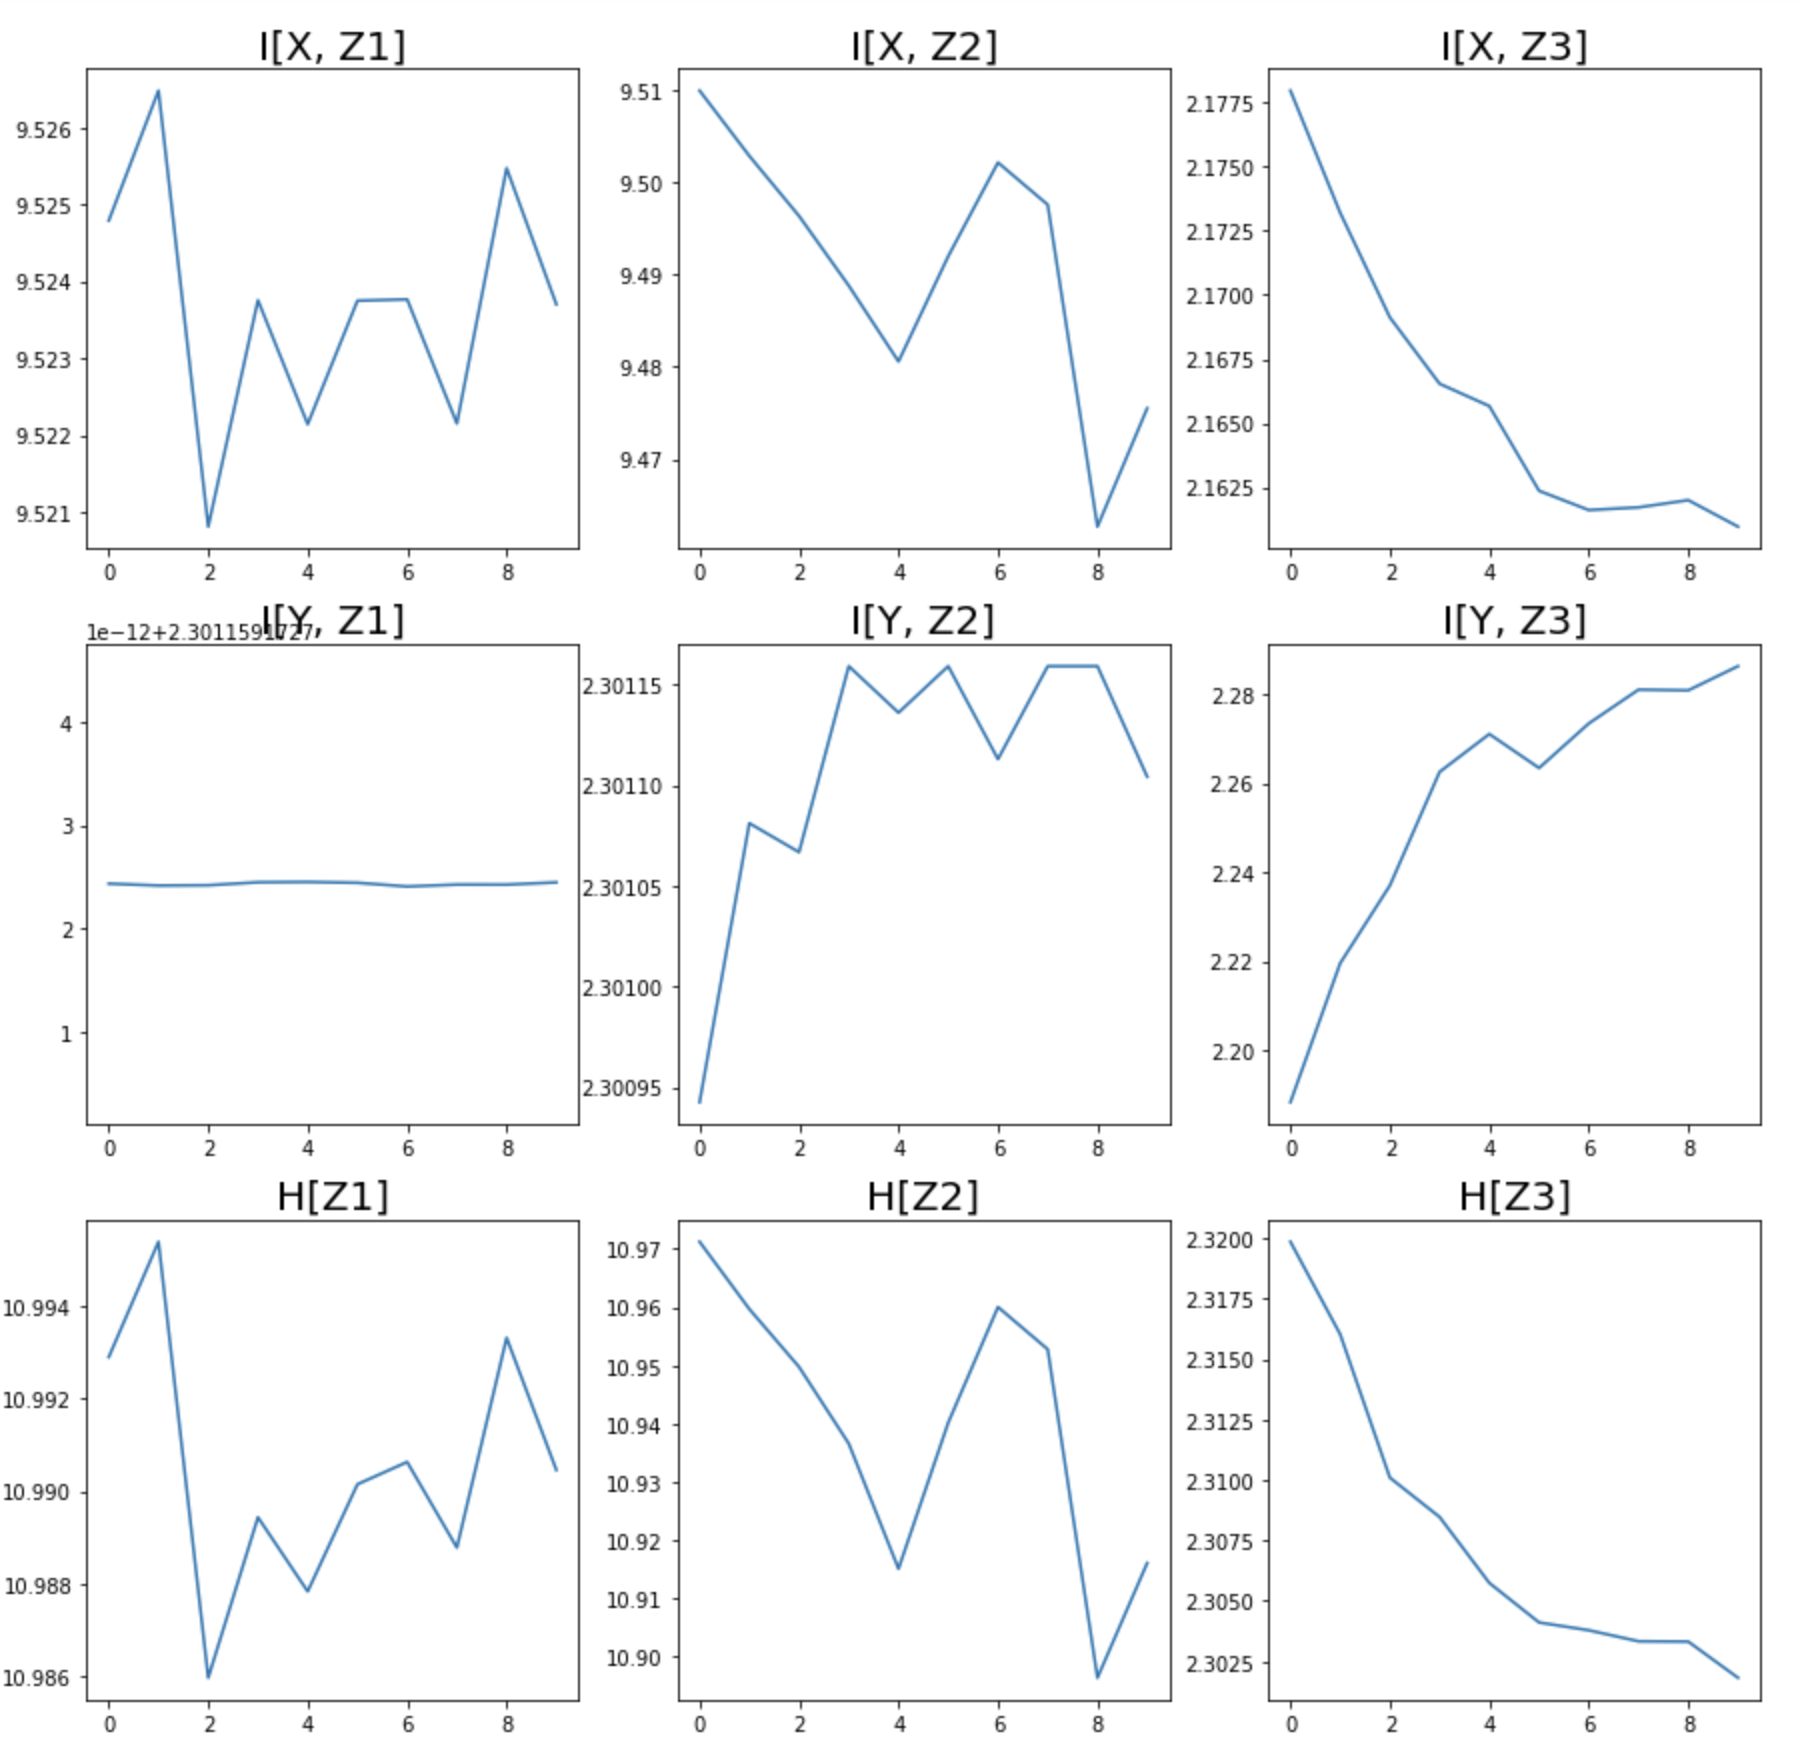
\includegraphics[scale=0.5]{images/inf_comp_v1.png}
\end{center} 

Здесь в данном примере в качестве гиперпараметров возьмем:
\begin{enumerate}
\item $waist\_input = MaxPool2d((4, 4))(input)$
\item $waist\_z1 = MaxPool3d((1, 4, 4))(z1)$
\item $waist\_z2 = MaxPool3d((1, 3, 3))(z2)$
\item $waist\_z3 = Softmax(z3)$
\end{enumerate}
То есть в промежуточных латентных слоях не смешивались каналы между собой. \\
Здесь проще всего рассмотреть как ведут себя информация между входным пространством и латентным $I[X, Z]$ и энтропия латентных пространств $H[Z]$. Как видно на графике данные эвристики уменьшаюся по мере обучения, причем чем проще латентное пространство устроено тем более функция от эпохи монотонная. Например $I[X, Z_3]$ и $H[Z_3]$ имеют более выраженое уменьшение с увеличением эпохи чем аналогичные эвристики только для $Z_2$ и $Z_1$. Аналогичное можно сказать про информацию между выходом и латентными пространствами $I[Y, Z]$. Чем больше $Z_i$ тем более монотона устроена функция. Только при этом $I[X, Z$ уменьшается в то время как $I[Y, Z]$ увеличивается. Более выроженная монотонность происходит по причине что пространсво $Z_3$ устроено проще чем другие латентные пространства. $Softmax(z_3)$ стремится к $one\_hot(y)$ для любых соответсвующих $z_3 \in Z_3, & y \in Y$. Таким образом в хорошо обученной сети:
\begin{gather}
\begin{aligned}
I[Y, Z] = \sum_{i=0}^{len\_dataset}p_{YZ}(y=y_i, z=z_i) * \log(\frac{p_{YZ}(y=x_i, z=z_i)}{p_Y(y=y_i) * p_Z(z=z_i)}) \approx \\
\sum_{i=0}^{len\_dataset}p_Y(y=y_i) * \log(\frac{p_Y(y=y_i)}{p_Y(y=y_i) * p_Y(y=y_i)} = \\
- \sum_{i=0}^{len\_dataset}p_Y(y=y_i) * \log(p_Y(y=y_i)) = H(Y) \approx \\
\sum_{i=1}^{10}0.1 * \log(10) = \log(10) \approx 2.3
\end{aligned}
\end{gather}
Как видно в текущем примере $I[Y, Z]$ не достигает максимальной оценки. Увеличение метрики $I[Y, Z]$ и уменьшение метрики $I[X, Z]$ подтвержает нашу гипотезу что метрику Information Bottleneck можно использовать как лосс функции, так как функция $I[X, Z] - \beta * I[Z, Y], \beta > 0$ уменьшается с улучшением сети. При этом информационные метрики для $Z_1$ устроены самым непонятным образом. Это связано с тем что данное латентное пространство наиболее сложное, и в нем наибольшее количество параметров: 
\begin{enumerate}
\item $waist\_input.shape = (1, 7, 7) \Rightarrow len(input\_params) = 2^{1 * 7 * 7} = 2^{49}$
\item $waist\_z1.shape = (16, 3, 3) \Rightarrow len(z1\_params) = 2^{16 * 3 * 3} = 2^{144}$
\item $waist\_z2.shape = (32, 2, 2) \Rightarrow len(z2\_params) = 2^{32 * 2 * 2} = 2^{128}$
\item $waist\_z3.shape = (10) \Rightarrow len(z3\_params) = 2^{10}$
\end{enumerate}
\subsection{Валидация гиперпарметров}
Проведем несколько экспериментов, сравнив информационные метрики для различных вероятностных пространств. Для этого первым экспериментом смешаем каналы для пространств $Z_2$ и $Z_3$, то есть MaxPooling будет проводиться также и по каналам. Этот эксперимент имеет смысл, так как в предъидушем примере латентные пространства имеют слишком большую размерность и как вывод сложные информационные представления. Соответственно смешиваение по каналам позволит уменьшить размерность пространства. В еще одном примере уменьшение размерности пространства будем осуществлять засчет увеличение окна 2d свертк, это позволит не смешивать каналы между собой. Для этого рассмотрим 3 примера с другими сверками. \\
1 пример:
\begin{enumerate}
\item $waist\_input = MaxPool2d((4, 4))(input)$
\item $waist\_z1 = MaxPool3d((2, 4, 4))(z1)$
\item $waist\_z2 = MaxPool3d((2, 3, 3))(z2)$
\item $waist\_z3 = Softmax(z3)$
\end{enumerate}
2 пример:
\begin{enumerate}
\item $waist\_input = MaxPool2d((4, 4))(input)$
\item $waist\_z1 = MaxPool3d((4, 4, 4))(z1)$
\item $waist\_z2 = MaxPool3d((4, 3, 3))(z2)$
\item $waist\_z3 = Softmax(z3)$
\end{enumerate}
3 пример:
\begin{enumerate}
\item $waist\_input = MaxPool2d((4, 4))(input)$
\item $waist\_z1 = MaxPool3d((1, 7, 7))(z1)$
\item $waist\_z2 = MaxPool3d((1, 7, 7))(z2)$
\item $waist\_z3 = Softmax(z3)$
\end{enumerate}
и посчитаем для новых вероятностных пространств информационные метрики.
Примеры 1-3 расположены слева направа на графиках.
\begin{figure}[!htb]
\minipage{0.33\textwidth}
  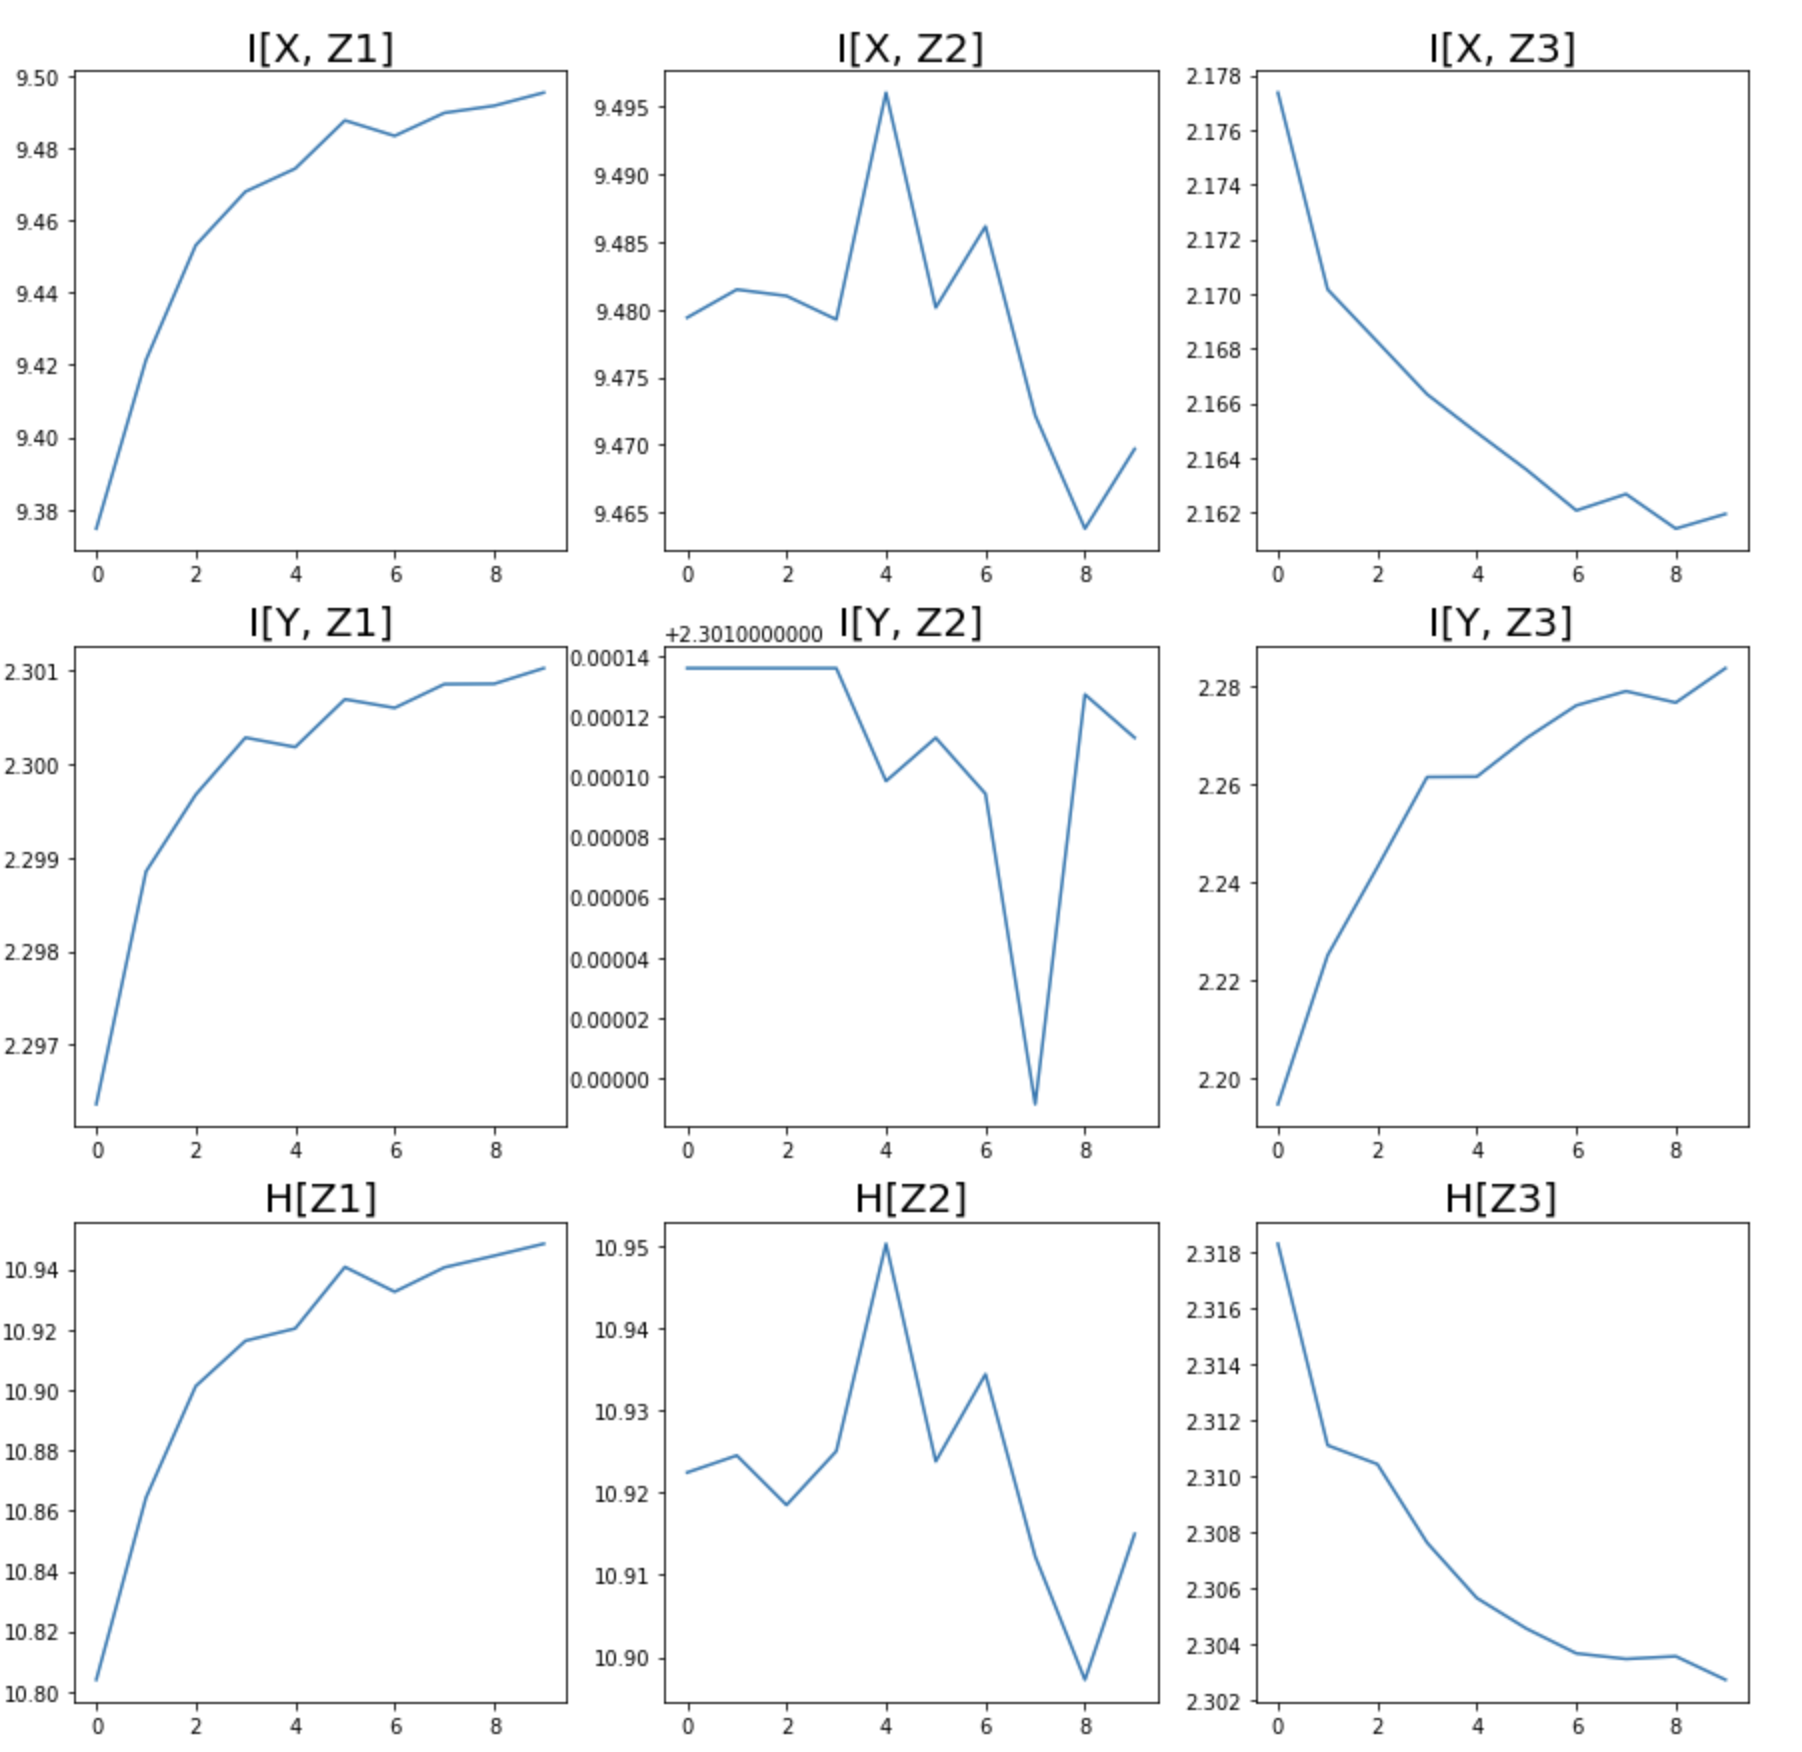
\includegraphics[width=\linewidth]{images/v2.png}
  
\endminipage\hfill
\minipage{0.33\textwidth}
  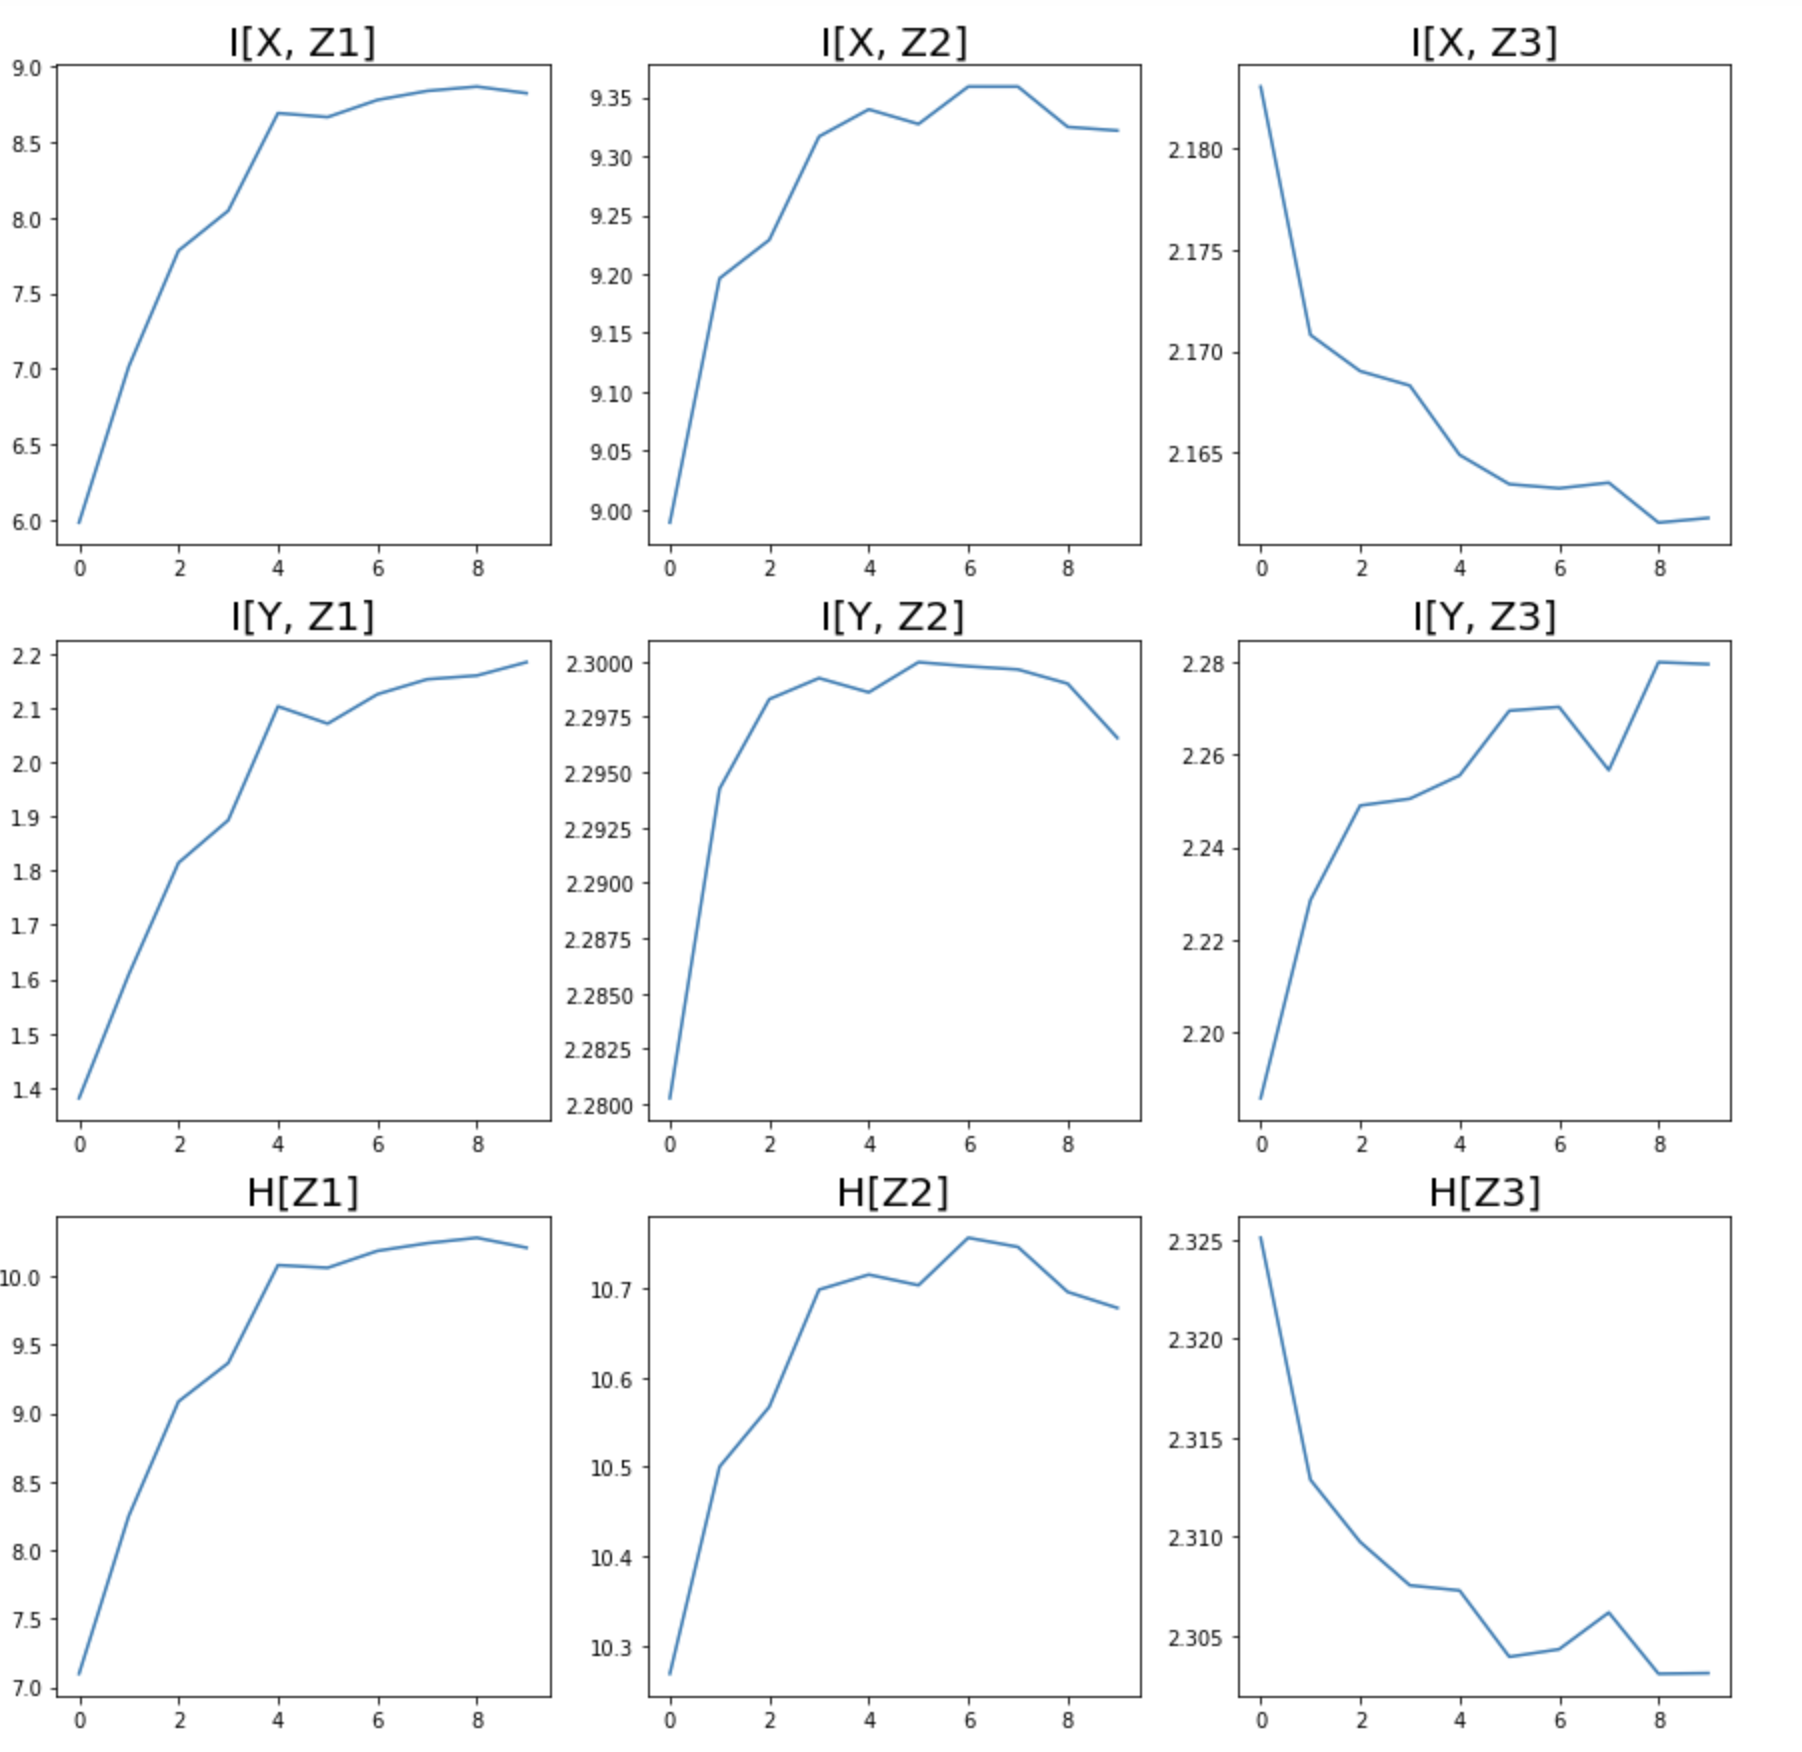
\includegraphics[width=\linewidth]{images/v3.png}
  
\endminipage\hfill
\minipage{0.33\textwidth}
  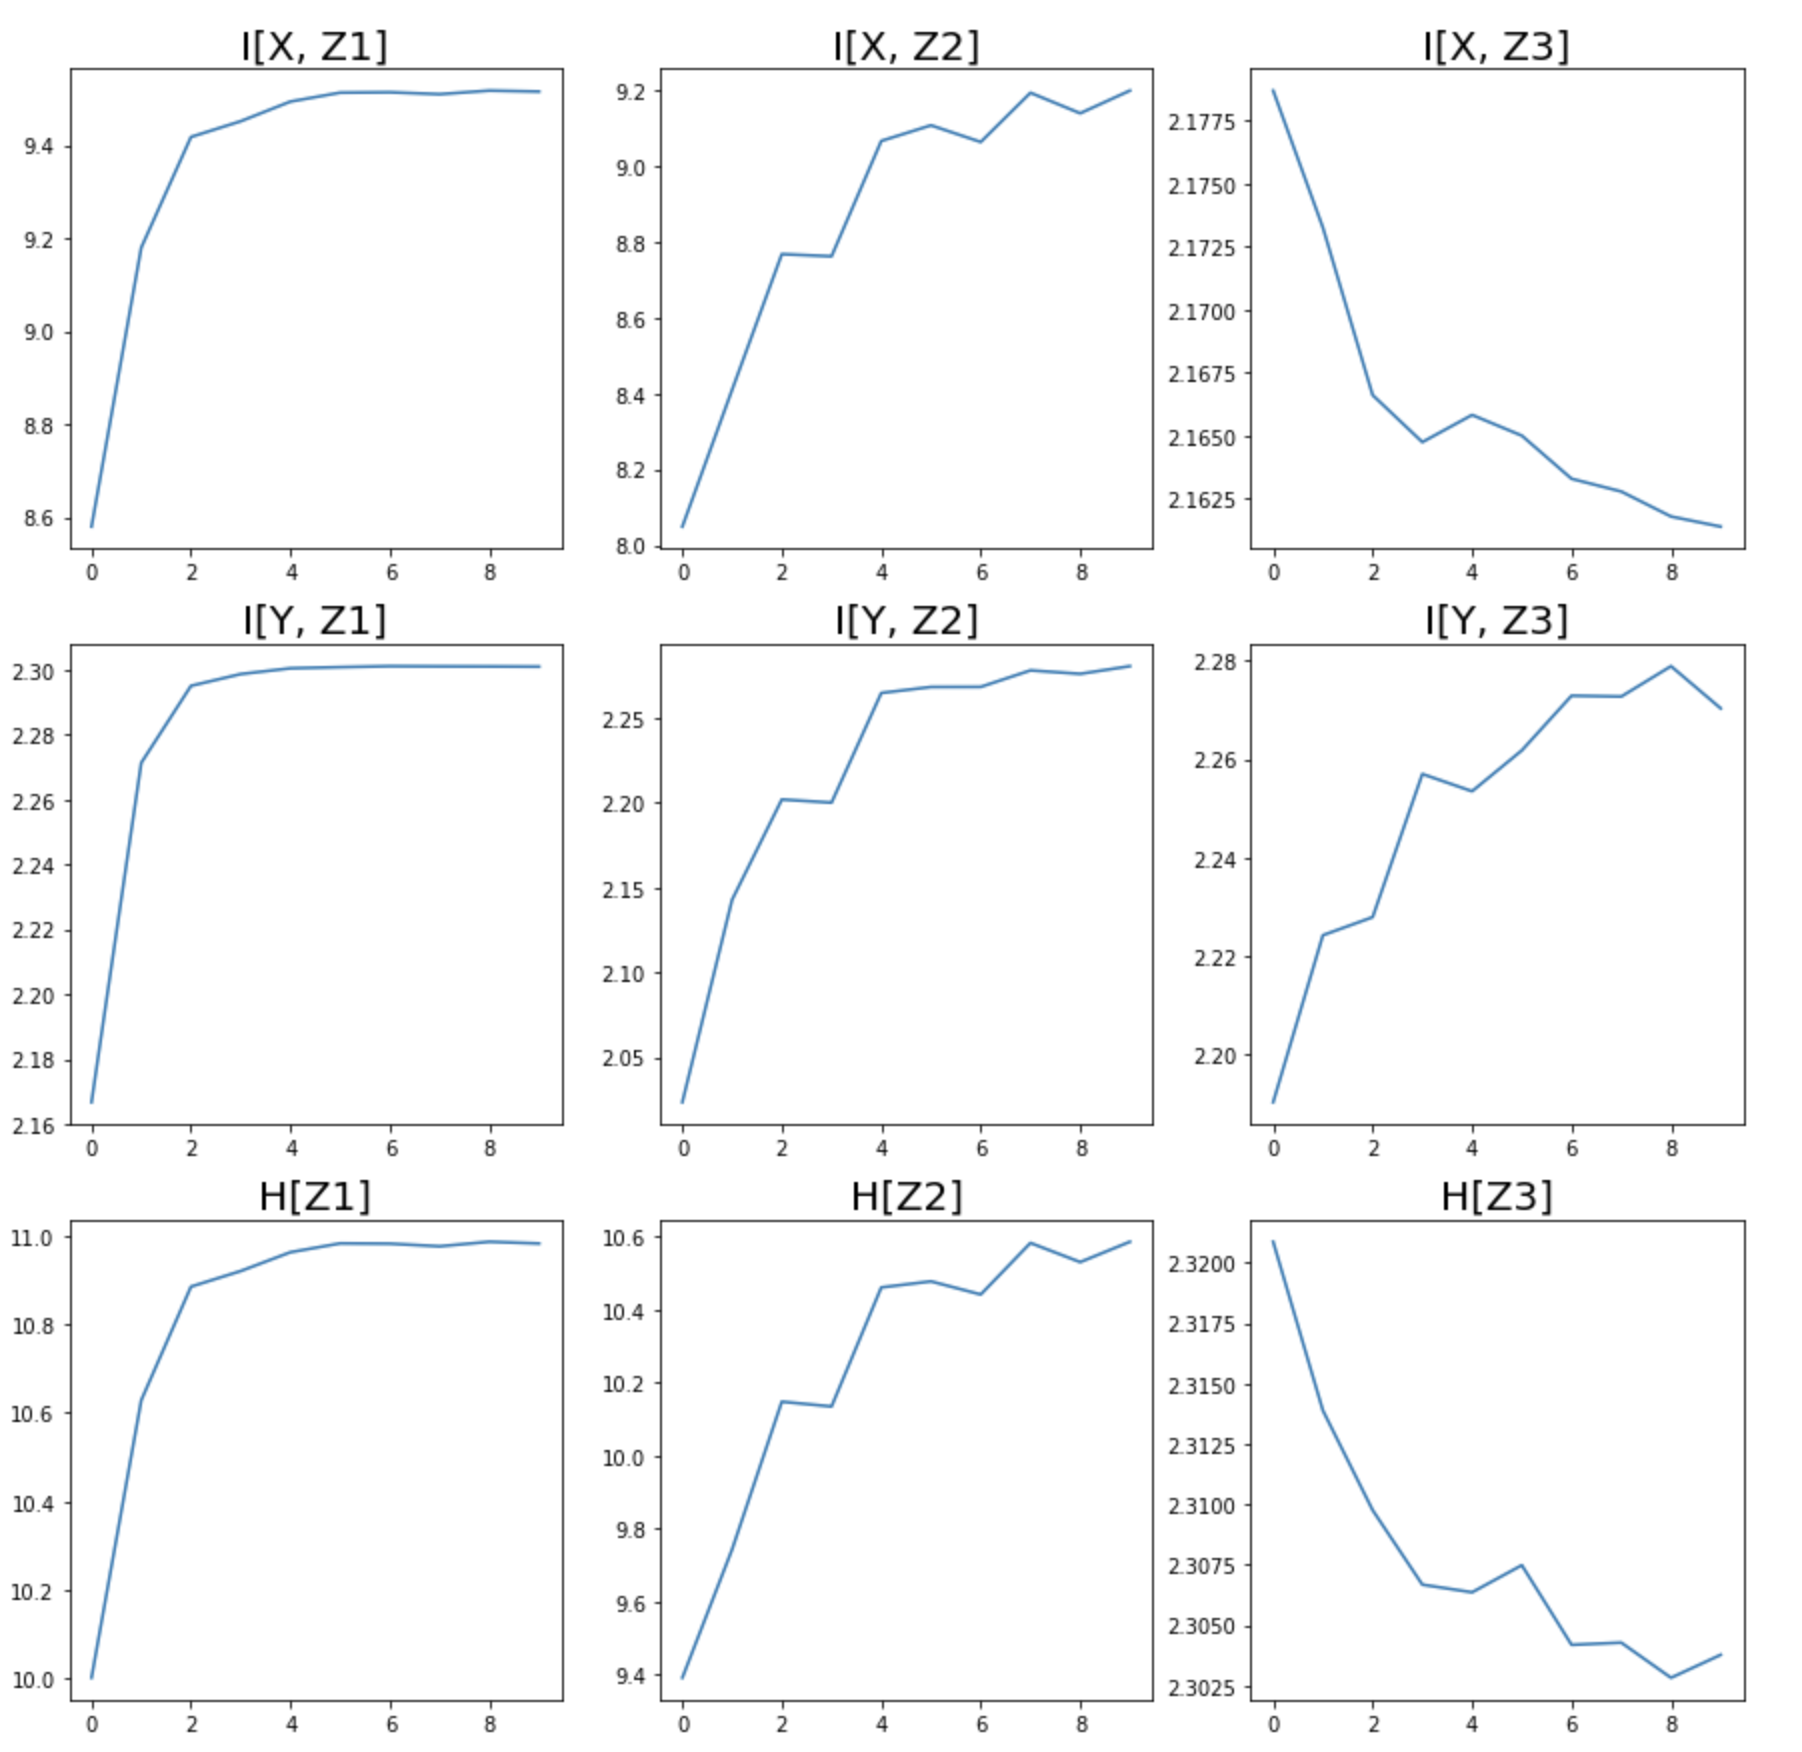
\includegraphics[width=\linewidth]{images/v4.png}
  
\endminipage
\end{figure}
Первое на что стоит обратить внивание - это возрастание метрики $I[X, Z]$ для всех примеров. Аналогично возрастает $I[Z]$. Это происходит по той причине, что значения на латентных слоях в обученных сетках распределены более равномерно. Это происходит по причине, что в необученной сети значения с большим значениями имеют большую вероятность в отличие от значений с маленькими значениями. Это происходит потому что беря максимум по окну с равномерно распределенными значениями максимум будет с большей вероятностью иметь большие значения
\begin{gather}
\begin{aligned}
X_{max} = max(X_1, X_2, ... X_n)
\end{aligned}
\end{gather}
где $X_i$ независимо одинаково распределеные случайные велечины. $X_i \in Uniform(0, 1)$, тогда 
\begin{gather}
\begin{aligned}
p(X_{max} < \alpha) = p(X_1 < \alpha) * ... * p(X_n < \alpha) = \alpha^{n} \rightarrow 0
\end{aligned}
\end{gather}
Соответветственно брав максимум по большому окну со смешанными каналами на плохо обученной сети расределение будет неравномерным. При обучении сети исходные латентные пространства имеют более выраженные предсавления: разрешенная матрица, где ненулевые значения обозначают реакцию на конкретные свертки - соответственно брав максимум по большому окну между несколькими каналами на выходе получится наибольшая реакция на свертку, что имеет равномерное распределение, поэтому с увеличением эпохи энтропия увеличивается и как следствие $H[Z]$ и $I[X, Z]$. Соответственно для данных гиперпараметров метика IB не будет уменьшаться с увеличением эпохи. \\
Для разрешение проблемы неравномерного распределения воспользуемся не maxpooling а avgpooling, то есть будем усреднять а не максимизировать значения в окне. При усреднении неравенство (26) уже не будет действовать, более того среднее у размеренной матрицы стремится к 0, соответственно ситуация с энтропией должны быть симетрична как в прошлом случае. Построим новый пример с нарда новыми гиперпараметрами. \\
4 пример:
\begin{enumerate}
\item $waist\_input = MaxPool2d((4, 4))(input)$
\item $waist\_z1 = ArgPool3d((1, 7, 7))(z1)$
\item $waist\_z2 = ArgPool3d((1, 7, 7))(z2)$
\item $waist\_z3 = Softmax(z3)$
\end{enumerate}
Расмтрим для данного эксперимента полученную информационную маску
\begin{center}
    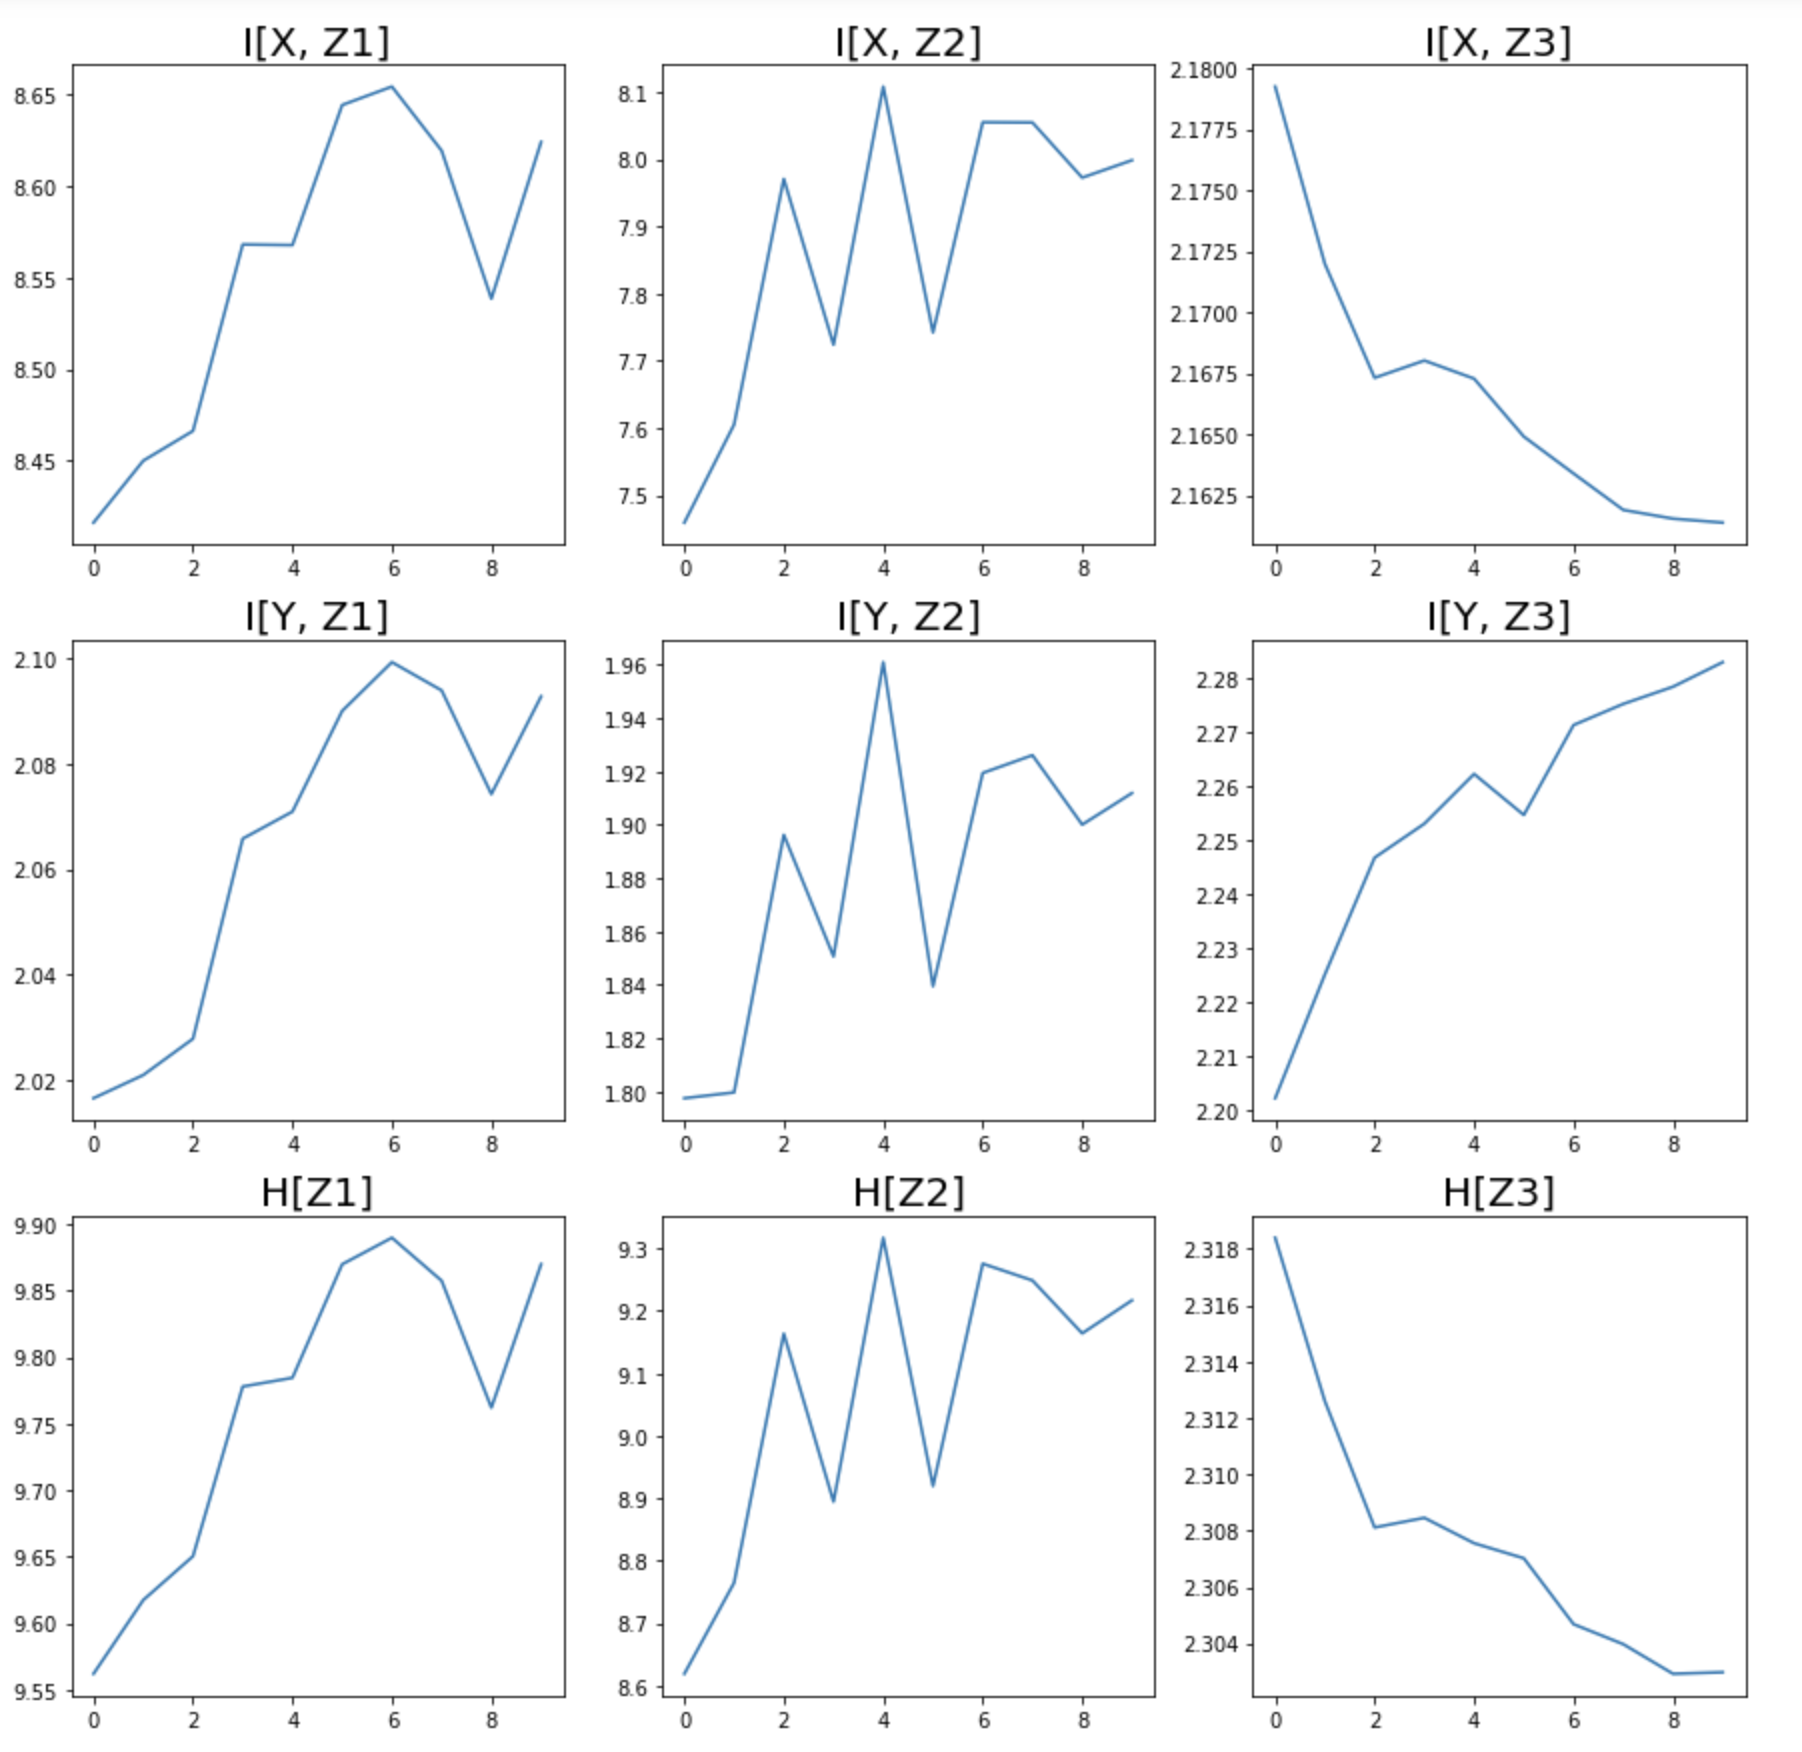
\includegraphics[scale=0.45]{images/v5.png}
\end{center}
Заметим, что возрастание функций $I[X, Z]$ и $I[Z]$ стало менее мнотонно, но при этом общий характер возрастания при увеличении эпохи остался, что требует большего изучения.
